\documentclass[a4paper,preprint,10pt,natbib,authoryear,onecolumn,prodmode,acmtoplas]{acmsmall}
\newif\iflong
\longtrue
\def\itemadjust{}
\usepackage{RR-white}
\usepackage[table]{xcolor}
\usepackage[greek,english,american]{babel}
%\usepackage[utf8]{inputenc}
\usepackage{natbib}
%\usepackage[chapter]{smartref}
\newcommand{\smartref}[1]{\ref{#1}}
\usepackage{chngcntr}
\usepackage{MnSymbol}
\usepackage{bbding}
%\counterwithout{section}{chapter}
\usepackage[hyperindex]{hyperref}
\hypersetup{
    pdftitle={Futex based locks for C11's generic atomics},
    pdfauthor={Jens Gustedt},
    pdfkeywords={lock primitives, atomics, C11, futex, Linux},
    pdfsubject={Futex based locks for C11's generic atomics},
    bookmarksopen = true,
    pdflang={English},
}
\usepackage{amsmath}
\usepackage[normalem]{ulem}
\usepackage{environ}
%\usepackage[T1]{fontenc}
%\usepackage{tipa}
%\usepackage{ucs}
%\SetUnicodeOption{tipa}
%\SetUnicodeOption{autogenerated}
\usepackage[euler]{textgreek}
\usepackage[utf8x]{inputenc}
%\usepackage{eurosym}
\usepackage{xspace, graphicx, subfigure, figlatex, array, multirow}
%\usepackage{amssymb}
\usepackage{url}
\usepackage{enumitem}
\usepackage[all,cmtip]{xy}
\usepackage{texgraphicx}% Pour inclure les pstex_t
\graphicspath{{./fig/}}
\usepackage{stfloats}
\usepackage{framed}
\usepackage{footmisc}
\definecolor{light-gray}{gray}{0.97}
%\usepackage{showlabels}
\usepackage{rotating}
\usepackage{fancybox}
\usepackage{etextools}
\usepackage{etoolbox}
\usepackage{placeins}
\setcounter{tocdepth}{2}

%\includeonly{cognition}
%\includeonly{}

% program listings
\usepackage{listings}
\usepackage{lstmisc}
\usepackage{titletoc}
\contentsuse{lstlisting}{lol}
\titlecontents{lstlisting}[2em]
              {\addvspace{0.25pc}}
              {\textbf{\lstlistingname~\thecontentslabel:} }
              {}
              {\titlerule*[0.5em]{$\cdot$}\contentspage}
              []
\usepackage{listings}
\usepackage{listings-C}
\usepackage{listings-x86_64}
\usepackage{listings-modernC}
\lstloadlanguages{C11,C99}
\lstset{
language=[errnoPOSIX]{C},
language=[tgmath]{C},
language=[threads]{C},
language=[stdatomic]{C},
language=[boundschecking]{C},
language=[99]{C},
language={C11},
style=modernC,
basicstyle=\tt\small,
moreemph=[5]{
futex_wait,
futex_wake,
},
moreemph=[3]{
smpl_lock,
smpl_unlock,
smpl, ftx,
ftx_cmpxch,
ftx_fetch_add,
ftx_fetch_sub,
ftx_lkd,
ftx_load,
ftx_lock,
ftx_set,
ftx_unlock,
},
}

\AtBeginDocument{\setlength{\tempdimen}{\textwidth}}
\lstloadlanguages{C11,C99}
\lstset{
  language=[errnoPOSIX]{C},
  language=[tgmath]{C},
  language=[threads]{C},
  language=[stdatomic]{C},
  language=[boundschecking]{C},
  language=[99]{C},
  language={C11},
  style=modernC,
  %basicstyle=\tt\footnotesize,
  moreemph=[5]{
    CMOD,
    alias,
    complete,
    declaration,
    defexp,
    definition,
    fill,
    slot,
    import,
    init,
    entry,
    link,
    mimic,
    module,
    none,
    separator,
    snippet,
  },
}
\makeatletter
\DeclareRobustCommand*{\escapeus}[1]{%
  \begingroup\@activeus\scantokens{#1\endinput}\endgroup}
\begingroup\lccode`\~=`\_\relax
   \lowercase{\endgroup\def\@activeus{\catcode`\_=\active \let~\_}}
\makeatother
\newcommand{\code}[1]{\text{\lstinline`#1`\xspace}}
\newcommand{\aode}[1]{\text{\lstinline[language={[x86_64]Assembler}]{#1}\xspace}}
\def\basename#1{%
  \csname filename@parse\endcsname{#1}%
  \csname filename@base\endcsname.\csname filename@ext\endcsname%
}
\newcommand{\lstpartial}[4][]{%
  \par%\vspace*{-3ex}%\noindent\vbox{%
    \lstinputlisting[%
    nolol,%
    firstline=#2,%
    firstnumber=#2,%
    lastline=#3,%
    title={\hbox to \linewidth{\footnotesize\hfill\fcolorbox{gray}{light-gray}{\escapeus{\basename{#4}}}}},%
    belowcaptionskip={0.8ex},%
    abovecaptionskip={-.5ex},%
    #1%
    ]%
    {#4}%
  }%}
\newcommand{\lstextract}[4][]{%
  %\marginpar{#4}
  \par{%
    \def\label##1{}%
    \lstinputlisting[%
    nolol,%
    firstline=#2,%
    firstnumber=#2,%
    lastline=#3,%
    title={\hbox to \linewidth{\footnotesize\hfill\fcolorbox{gray}{light-gray}{\escapeus{\basename{#4}}}}},%
    belowcaptionskip={0.8ex},%
    abovecaptionskip={-.5ex},%
    #1%
    ]%
    {#4}%
  }}
\newcommand{\lstget}[4][]{%
  %\marginpar{#4}
  \par{%
    \def\label##1{}%
    \lstinputlisting[%
    nolol,%
    firstline=#2,%
    firstnumber=#2,%
    lastline=#3,%
    caption={},%
    backgroundcolor={},%
    #1%
    ]%
    {#4}%
  }}
\newcommand{\lstassembler}[4][]{%
  \par%
    \lstinputlisting[%
    language={[x86_64]Assembler},%
    nolol,%
    firstline=#2,%
    firstnumber=#2,%
    lastline=#3,%
    title={\hbox to \linewidth{\footnotesize\hfill\fcolorbox{gray}{light-gray}{\escapeus{\basename{#4}}}}},%
    belowcaptionskip={0.8ex},%
    abovecaptionskip={-.5ex},%
    #1%
    ]%
    {#4}%
  }
\def\textexclam{!}
% program output
\usepackage{fancyvrb}
\renewcommand{\FancyVerbFormatLine}[1]{%
  \colorbox{light-gray}{\hbox to 0.95\linewidth{#1\hfill}}%
}
\DefineVerbatimEnvironment%
{TerminalX}{Verbatim}
{
%commandchars=\\\{\},
firstnumber=0,
samepage=true,
fontsize=\footnotesize,
numbers=left,
numbersep=2mm,
label=\raisebox{0.6ex}[2ex][0ex]{\fcolorbox{black}{light-gray}{\small Terminal}},
frame=single,
fillcolor=\color{light-gray},
framesep=1em
}
\newenvironment{terminal}
  {\VerbatimEnvironment
   \vspace*{1ex}
   \TerminalX}
  {\endTerminalX}


\usepackage{fmtcount}
% \def\hechs#1{
%   %\def\ARG{\arabic{#1}}%
%   \ifthenelse{#1<10}{\arabic{#1}}{\alph{#1}}
%   %\alph{#1}
% }
% \renewcommand{\thesection}{\hexadecimal{section}}
% \renewcommand{\thesubsection}{\thesection.\hexadecimal{subsection}}
% \renewcommand{\thesubsubsection}{\thesubsection.\hexadecimal{subsubsection}}

%\newcommand{\shortchaptername}{Lev.}
% indexing
\newcommand{\specindex}[2][]{%
  \expandafter\newcommand\csname#2index\endcsname[2][]{%
    \def\CAT{#1}%
    \ifx\CAT\empty%
    \else%
    \def\CAT{|#1}%
    \fi%
    \def\ARG{##1}%
    \ifx\ARG\empty%
    \index{##2\CAT}%
    \else%
    \index{##1\CAT}%
    \fi%
    \csname#2\endcsname{##2}\noexpand\xspace%
  }%
}
\specindex[textbf]{emph}
\newcommand{\jargon}[1]{{\bf\em #1}$^{C}$}
\specindex{jargon}
\newcommand{\plain}[1]{#1}
\specindex{plain}

\def\footwarmmark{[Exs~\arabic{footnote}]}
%\newtheorem{exs}{Exercise}
\makeatletter
\def\blfootnote{\xdef\@thefnmark{\footwarmmark}\@footnotetext}
\makeatother
\newcommand{\footwarm}[2][]{%
  \def\ARG{#1}%
  \ifx\ARG\empty%
  \else%
  \def\ARG{\label{#1}}%
  \fi%
  \addtocounter{footnote}{1}%
  ${}^{\text{\footwarmmark}}$\blfootnote{\ARG\ #2}%
}

\newcommand{\STDC}[3][]{
  \def\ARG{#1}%
  \ifx\ARG\empty%
  \def\ARG{9899:2011}%
  \fi%
  \def\PAR{#3}%
  \ifx\PAR\empty%
  \else
  \def\PAR{~#3}%
  \fi%
  ISO~\ARG~#2\PAR\xspace
}
% \newtheoremstyle{common}
%     {0ex}% above space
%     {0ex}% below space
%     {\itshape}% body font
%     {0em}% indent
%     {\begin{tabular}{l}\cellcolor{yellow}}% head font
%     {\end{tabular}}% punct after head
%     {.5em}% space
%     {}% custom
% \theoremstyle{common}
\newtheorem{remInder}{Rule}%[subsection]
\gdef\Arg{}%
\newcommand{\Reminder}[2][]{%
  \begin{remInder}%[#1]%
  \begin{minipage}[t]{0.8\linewidth}%
    #2%
  \end{minipage}%
  \end{remInder}%
  \def\Arg{#1}%
  \ifx\Arg\empty\let\Arg=\relax\else\def\Arg{\noexpand\noexpand\noexpand\marginpar{#1}}\fi%
  \addcontentsline{rem}{section}{\colorbox{yellow}{\hbox to
      3.5em{\theremInder}}\ #2\Arg}%
}
\NewEnviron{reminder}[1][]{%
  \removelastskip%
  \vskip 0.5ex plus 0.5ex minus 0.5ex%
    \Reminder[#1]{%
      \BODY%
    }%
  \vskip 0.5ex plus 0.5ex minus 0.5ex%
  %\ \hfill\\
}
\newcommand{\remindername}{Reminders}
\newcommand{\listofreminders}{
  \clearpage
  %\addcontentsline{toc}{chapter}{\remindername}
  \csname @starttoc\endcsname{rem}\remindername
}

\newcommand{\Cinclude}[1]{\texttt{#1}}

\newenvironment{annexpar}[1]{
  \pagebreak[2]
  \noindent\index{Annex #1}
  \ \marginpar{\mbox{\footnotesize Annex~#1}}\pagebreak[0]\\[-2ex]%
  \pagebreak[0]\noindent
  \definecolor{shadecolor}{named}{lightgray}
  \begin{shaded}
}{\end{shaded}}

\newenvironment{AnnexK}{\begin{annexpar}{K}}{\end{annexpar}}

\newenvironment{DoxyItemize}{\itemize}{\enditemize}
\newenvironment{DoxySeeAlso}[1]{\par\smallskip\textbf{#1}: }{\par}
\newenvironment{DoxyParams}[1]{\par\smallskip\textbf{#1}:\hfill%
  \tabular[t]{|l|p{8.5cm}|}\hline%
}
{\endtabular\par\bigskip}
\newenvironment{DoxyRemark}[1]{\par\smallskip\textbf{#1}: }{\par}
\newenvironment{DoxyReturn}[1]{\par\smallskip\textbf{#1}: }{\par}
\newcommand{\longPar}{\let\oPar=\par\def\par{\oPar\medskip\let\par=\oPar}}
\newenvironment{DoxyDocu}[1]{%
  \index{#1@\texttt{#1}}%
  \parindent=0pt%
  \longPar%
  \code{#1}: %
  \parskip=1ex%
}{}
\newcommand{\functionDocu}[4]{
  \def\FName{\escapeus{\basename{#4}}}%
  \par\medskip\noindent%
  \fcolorbox{gray}{light-gray}{
    \begin{minipage}[t]{0.97\linewidth}
      \hfill{\tiny \texttt{\FName}}\\%
      \input{code/snippets/#1}
      \par
      \lstinputlisting[%
      numbers=none,%
      frame=topline,%
      firstline=#2,%
      firstnumber=#2,%
      lastline=#3,%
      ]{#4}
    \end{minipage}
  }
  \medskip
}

%\newtheorem{definition}{Definition}
%\newtheorem{theorem}{Theorem}
%\newtheorem{lemma}{Lemma}
%\newtheorem{corollary}{Corollary}
% \conferenceinfo{CONF 'yy}{Month d--d, 20yy, City, ST, Country}
% \copyrightyear{2015}
% \copyrightdata{978-1-nnnn-nnnn-n/yy/mm}
% \doi{nnnnnnn.nnnnnnn}

\newcommand{\Prepro}{\ensuremath{\mathcal{P}}}
\newcommand{\Header}{\ensuremath{\mathcal{H}}}
\newcommand{\Decl}{\ensuremath{\mathcal{D}}}
\newcommand{\Impl}{\ensuremath{\mathcal{I}}}
\newcommand{\spare}{\mbox{\tiny\Plus}}


\makeatletter
\makeatother


\RRprojet{Camus}
\RCNancy
\RRdate{December 2015}

\begin{document}
%\terms{Languages; Standardization;}
%\acmVolume{subm.}
%\acmNumber{N}
%\acmArticle{\spare}
%\acmYear{2015}
%\acmMonth{6}
%\acmformat{Jens Gustedt. 2015. Modular C.}
%\markboth{Jens Gustedt}{Modular C}
%\maketitle

\RRNo{8818}
\RRetitle {Futex based locks for C11's generic atomics%
  \thanks{A short version of this paper is accepted for publication in SAC'16, see~\cite{gustedt16:futex}}
}
\RRauthor {Jens Gustedt%
\thanks[inria]{Inria, France}%
\thanks[uniS]{Universit\'{e} de Strasbourg, ICube, France}%
}
\RRtitle  {Verrous basés sur futex pour les opérations atomiques génériques de C11}
\titlehead{Futex based locks for C11's generic atomics}

% {jens gustedt inria fr}
%\urladdr{\url{http://icube-icps.unistra.fr/index.php/Jens\_Gustedt}}
%\preprintfooter{all rights reserved}   % 'preprint' option specified.
% \authorinfo{Geminus Caecus}
% {terra incongnita}
% {}
%\thanks{blabla ICube, Strasbourg, France}
% \keywords{}

\RRabstract {
  We present a new algorithm and implementation of a lock primitive that
is based on Linux' native lock interface, the \texttt{futex} system
call. It allows us to assemble compiler support for atomic data
structures that can not be handled through specific hardware
instructions.  Such an implementation is needed for C11's atomics
interface because here an \code{_Atomic} qualification can be attached
to almost any data type. Our lock data structure for that purpose
meets very specific criteria concerning its field of operation and its
performance. By that we are able to outperform gcc's
\texttt{libatomic} library by around 60\%.

%%% Local Variables:
%%% mode: latex
%%% mode: reftex
%%% fill-column: 75
%%% ispell-dictionary: "american"
%%% x-symbol-8bits: nil
%%% End:

}

\RRkeyword {lock primitives, atomics, C11, futex, Linux}

\RRresume{%
  Nous présentons un nouveau algorithme pour une primitive de verrouillage et
son implantation qui se basent sur l'interface natif de Linux, l'appel
système \texttt{futex}.
%
Ceci nous permet d'assembler le support à la compilation de structures de
données atomiques tant qu'il ne peut pas être réalisé par une instruction
matérielle.
%
Une tel outil est nécessaire pour l'interface atomique de C11, car ici la
qualification \code{_Atomic} peut être attribuée à presque tous les types de
données.
%
Notre structure de verrouillage vérifie des propriétés spécifiques pour son
champ opérationnel et ses besoins de performance.
%
Ainsi nous sommes en mesure surpasser les performances de la bibliothèque
\texttt{libatomic} de gcc par 60\%.

%%% Local Variables:
%%% mode: latex
%%% mode: reftex
%%% fill-column: 75
%%% ispell-dictionary: "french"
%%% x-symbol-8bits: nil
%%% End:

}

\RRmotcle {primitives de verrouillage, opérations atomiques, C11, futex, Linux}


\makeRR


\section{Introduction}
\label{sec-1}

Only very recently (with C11, see \citeauthor{C11}) the C language has
integrated threads and atomic operations into the core of the
language.  Support for these features is still partial: where the
main open source compilers~\citeauthor{gcc} and~\citeauthor{clang} now offer atomics, most Linux
platforms still use~\citeauthor{glibc}
as their C library which does not implement C11 threads. Only
platforms that are based on~\citeauthor{musl} as C
library, e.g~\citeauthor{alpine}, are
feature complete.

The implementation of the C11 atomic interface typically sits in the
middle between the implementation of the core language by the C
compiler and the implementation of the C library. It needs compiler
support for the individual atomic operations and library support for
the cases where no low-level atomic instruction is available and a
lock must be taken. We refer to the latter, as a \emph{generic atomic
lock} interface.

Since Linux' open source C libraries do not implement the generic
interface, the compilers currently provide a library stub that
implements the necessary lock by means of a combination of atomics
and~\citeauthor{POSIX2009}
\code{pthread_mutex_t}. By consensus in the community an API interface
has emerged that both, \texttt{gcc} and \texttt{clang}, implement.

This library stubs can rely on all their knowledge of the
architecture specific atomics for the non-contended part of the
implementation, finally that is the context in which they were
created. But since they are generic, in case of contention these
library stubs rely on generic OS interfaces to put threads to
sleep. From a point of view of the C language the natural interface
for that would be C11 threads, that could be a bit lighter than
POSIX threads. But since this end is still missing in \texttt{glibc}, they
fall back to POSIX threads for which there are reliable and
efficient implementations.

This situation is less than ideal, the role of a language interface
is finally to do the work of mapping to platform specific properties
and thereby to draw the best performance from any given hardware. In
this work we present a specific algorithm for the generic lock that
relies on a specific set of Linux utilities, the \texttt{futex} system
calls. These system calls combine just one atomic integer and OS
scheduling in a very ingenious way and are the tool of choice of a
Linux specific implementation of any lock structure.

Our algorithm uses all possibilities that the \texttt{futex} interfaces
offers. In particular we use just one \code{unsigned} integer to
implement the lock and a waiter count at the same time. Not only is
the resulting data type of minimal size (32 bit on all
architectures) but the algorithm can take advantage of that property
by minimizing the number of CPU to memory transfers. In most cases
one such transfer is sufficient, where other algorithms have to
update a lock and a waiter counter separately.

To our knowledge pursuing this approach to a complete solution is
new. Previously urban myth had it that such approaches would risk
deadlocks if confronted to heavy load, because repeated failures of
calls to \code{futex_wait} could lead to unbounded loops. We are able to
prove that such unbounded loops will not happen for our algorithm.
Also, our measurements have shown that such an approach can be very
effective: failed system calls to \code{futex_wait} are much less costly
than commonly thought.

Our algorithm and its implementation is part of a larger open
source project to provide the necessary interfaces (header files)
and library support for C11's \code{<stdatomic.h>}. Unfortunately, due to
space limitations we will not be able to present this project
further, but have to concentrate on the generic lock feature that it
provides.

At the time of this writing this project is functional to be used
with \texttt{gcc} and \texttt{clang}, even for version that only have partial
support for atomic operations through builtin functions. If accepted
for publication, we will provide links to the complete source in the
de-anonymized version. In a later stage, we intent to integrate the
whole project into the \texttt{musl} C library.

\section{Tools to deal with data consistency and races}
\label{sec-2}

Data races are the most difficult challenge for parallel
programming. They often lead to hard to trace sporadic errors. The
main problems are:\itemadjust

\begin{description}
\item[{atomicity:}] Writes to memory may or may be not split by the
hardware into several chunks that are written
separately. A reader may occasionally see
inconsistent values, for example a high and a low
word of a wide integer that originate from different
writes.\itemadjust
\item[{divisibility:}] A read-modify-write operations such as a simple
\code{i++} may be split into several CPU instructions,
e.g a read, an increment and a write. If a first
write of another threads falls sometime between
the read and the write, the new write will erase
the value with one that is outdated.\itemadjust
\item[{memory ordering:}] The results of read and writes to different
objects in memory might be perceived by different threads in
different order. Reordering of instructions may originate from
optimization (compiler) or occur at run time (processor).
\end{description}

\itemadjust
A data type that is guaranteed to avoid the first problem is called
\emph{atomic}. Before the C11 revision C only had one data type,
\code{sig_atomic_t}, that had this guaranty to be read and written in one
chunk. It can be used to communicate state between a user program
and a signal handler.

For the second problem, divisibility, C had no standard tool. No
other operation than read or write of \code{sig_atomic_t} was guaranteed
to be \emph{indivisible}.  The \emph{indivisible} operations that most
computing hardware offer could not be accessed through language
features. Usually they had to be programmed through extensions such
as inline assembler or special compiler builtins.

Before C11, C also had no thread concept, so the memory ordering
problem could not even be formalized within the vocabulary of the C
standard. Obviously, it also could not provide tools to deal with
it.

\subsection{C atomics and its library interfaces}
\label{sec-2-1}

With modern multi-processor and multi-core hardware, parallel
programming is an imperative for many if not most user applications
that are used on a larger scale. Therefore it was crucial for C to
provide the concepts and tools that are necessary to deal with
it. So C11 introduces a lot of vocabulary and two optional
features: threads through the \code{<threads.h>} interface, and atomics
trough the \code{<stdatomic.h>} interface. Evidently here we are more
interested in the latter, but it is important to note that both
features need each other to unfold all of their potential.

C11 introduced a new qualifier, \code{_Atomic}. A such qualified object
guarantees that any read or write access to it is \emph{atomic} in the
sense we have defined above. This qualification also guarantees
that between different threads all standard operations (defined
through operators such as \code{+=} or functional such as
\code{atomic_exchange}) are perceived as \emph{indivisible}. Note well that
this guarantee is only given \emph{between threads} and \emph{in perception}:
in reality an operation can well be divided into several processor
instructions and the perception guarantee does not extend to
visibility between the main program and signal handlers. An
operation that extends perception of indivisibility to signal
handlers is called \emph{lockfree} in the jargon of the C
standard. Below we will see where this choice of words originates.

C11 also introduces different concepts of \code{memory_order} for atomic
operations. The whole of that specification is much too complex to
unfold, here. In the following we will assume \emph{sequential
consistency} (\code{memory_order_seq_cst}) for all atomic
operations. This forces all atomic operations to appear totally
ordered between all threads.

We will use the following atomic operations:
\itemadjust
\begin{itemize}
\item[] \hspace*{-3ex}\code{atomic_store}: store a new value
\itemadjust
\item[] \hspace*{-3ex}\code{atomic_exchange}: store a new value and
 return previous
\itemadjust
\item[] \hspace*{-3ex}\code{atomic_fetch_add}: add value and
 return previous
\itemadjust
\item[] \hspace*{-3ex}\code{atomic_fetch_sub}: subtract value and
 return previous
\itemadjust
\item[] \hspace*{-3ex}\code{atomic_compare_exchange_weak}: compare to desired, then
  exchange, may fail
\end{itemize}




\subsection{Atomic instructions on modern hardware}
\label{sec-2-2}

Almost since the beginning of modern computing, parallelism was
implemented in hardware and the consistency problems that we
introduced above became apparent
\iflong
.
An early overview of the problem had been given by
\else
,
see \textsl{e.g.}
\fi
\cite{Netzer1992}.
Modern hardware (which almost
always is inherently parallel) deals with this by providing special
instructions, usually referred to as \emph{atomic instructions}. It is
important to note that these are not the same as the atomic
operations on the level of the C language.\itemadjust

\begin{description}
\item[{word size:}] Usually atomic instructions are limited to word
sized data types. Available on most platforms are
instructions for 8, 16, 32 and 64 bit
data types. Some also extend to 128 bit.\itemadjust
\item[{primitives:}] The instructions that are implemented may or may
not directly correspond to atomic operations. E.g
some CPU may have a proper instruction for the
increment operator \code{++}, e.g \texttt{x86\_64}, on others,
e.g \texttt{arm}, such an operation will have to be
composed from primitives.\itemadjust
\item[{boundedness:}] Atomic instructions may give a guarantee to
succeed within a bounded time (usually some
memory cycles) or just return success or
failure. For the latter, this may result in C
level operations that have an \emph{unbounded}
response time.\itemadjust
\item[{state:}] Atomic instructions may operate on an internal state of
the platform. E.g \texttt{arm} CPU work with a feature called
\emph{monitors} that memorize state of previous atomic
access to memory.\itemadjust
\end{description}

Due to all these differences, programming with atomic instructions
directly on assembly level is a mess, and in general it is very
tedious to provide portability between different
architectures. Such code has to ensure\itemadjust
\begin{itemize}
\item the correct composition of atomic primitives to obtain sensible
semantics of the operations,\itemadjust
\item the correct alignment of all atomic object such that they do not
cross cache line boundaries,\itemadjust
\item the correct ordering of instructions, e.g it has to ensure that
neighboring store instructions are not reordered by the CPU,
\itemadjust
\item that the unboundedness of some operation may not result in
application deadlocks,\itemadjust
\item and that the OS correctly restores processor state when the
execution context switches from one thread to another or to a
signal handler.
\end{itemize}

Luckily, C11 now ensures that only C compiler and C library
Implementers have to consider all the glorious details of a
specific architecture. One problem remains though, and this is what
this paper is all about. Because of the limited word size for
atomic instructions, the implemented compiler operations cannot just
resort to a composition of atomic primitives on the atomic object
itself. If an object is large, say 128 bit wide, or has a size that
is not a power of 2, they must rely on external or internal \emph{locks}
that protect a \emph{critical section}, CS. That is they need an
auxiliary object that protects the data object by means of some
\emph{lock primitives} and by memorizing a \emph{state} of the application.

Typically such locks can be made invisible between different
threads, but remain visible between a thread and its signal
handler. So the access to an object that is qualified with
\code{_Atomic} but that needs a lock for operation may be divisible with
respect to a signal handler. This property is what coined C's
terminology of \emph{lockfree} that we already mentioned above.


\subsection{Fast user space mutexes}
\label{sec-2-3}

In a singular toolbox \emph{Fast User space muTEXes}, \texttt{futex} for
short, the Linux kernel combines two levels of operations for the
implementation of lock primitives, see
\cite{Hutton02fuss,hart09}:\itemadjust

\begin{enumerate}
\item User space atomic integers with lockfree operations are used to
regulate access to the lock as long as it is not congested.\itemadjust

\item Wait and wake-up system calls resolve conflicts when the lock is
under congestion by multiple threads or processes. They relate
to such integers by address (user space or kernel space
addresses) and are guaranteed to be perceived as indivisible by
the caller.\itemadjust
\end{enumerate}

In the beginning, when \texttt{futex} were first introduced they needed
non-standard features: assembly extensions for the atomic
instructions, and a system call interface into the Linux
kernel. Fortunately with the atomics interface of C11 we now have
a standardized tool for the first. For the second, in the
following we will assume that we have two library calls
\code{futex_wait} and \code{futex_wake} at our disposal.
%
This is only a very restricted set of the available futex operations that
is simple to master and avoids most of the complexity of the interface as
it was described by~\cite{drepper11:futex}. The only difficulty that
remains is that a call to \code{futex_wait} is only successful if the
kernel can guarantee that the value of the atomic object still is as
expected.
%
With these interfaces a simple but
inefficient lock structure \code{smpl} could look as follows:

\lstset{language=C11,label= ,caption= ,numbers=none}
\begin{lstlisting}
typedef _Atomic(int) smpl;
void smpl_lock(smpl* lck) {
 for (;;) {
  int prev = atomic_exchange(lck, 1);
  if (!prev) break;
  futex_wait(lck, prev);
 }
}
void smpl_unlock(smpl* lck) {
 atomic_store(lck, 0);
 futex_wake(lck, 1);
}
\end{lstlisting}

Here the second parameter to \code{futex_wait} guarantees that the thread
will only be set to sleep if the value of the atomic object \code{*lck}
still is \code{prev}. As a consequence the \code{smpl_lock} function will iterate until the
atomic exchange succeeds in modifying the value from a previous
value of \code{0} to the value of \code{1}.

The second parameter of \code{futex_wake} corresponds to the maximal
number of threads that are to be woken up. So here, the thread that
holds the lock restores the object \code{*lck} to the value \code{0} and wakes
up one possible waiter.

Both functions as described above are simplistic and not very
efficient. The first, \code{smpl_lock}, is inefficient because each failed
attempt to acquire the lock will result in a call into the OS
kernel, even if the lock would be available almost instantly.  The
second, \code{smpl_unlock}, tries to wake up another thread without any
knowledge if there even is such a thread that is waiting for it.

To avoid these two shortcomings, system libraries that implement
locks (such as e.g \code{glibc} and \code{musl}) usually combine two
strategies:\itemadjust

\begin{itemize}
\item A first spinning phase attempts the atomic operation several
times. Thereby an application with a very short CS can mostly
avoid sending threads into sleep.\itemadjust

\item They use at least two \code{_Atomic} objects, one for the lock itself
and a second one that counts the waiters. By checking if the
counter is 0, this allows to avoid useless calls to
\code{futex_wake}.\itemadjust
\end{itemize}

Even though these additions enlarge the lock data structure and add
one atomic operation to the unlock function these strategies have
proven to be much more efficient then our simplistic versions,
above.

\section{A new generic lock algorithm using futex system calls}
\label{sec-3}

To construct and adapted lock data structure for our situation, we
want to have the following properties:

\begin{itemize}
\item The size of the data structure should be minimal. That is should
use just one 32 bit machine word as it is needed by the \texttt{futex}
calls.\itemadjust

\item When there is no contention, the number of atomic operations should
be minimal. That is one such operation for each, \code{lock} and
\code{unlock}, should suffice in that case.\itemadjust

\item The procedure should be efficient, that is it should not
unnecessarily waste resources. In particular, threads that have no
chance to acquire the lock should be put into an OS sleep
state.\itemadjust

\item If the number of threads is bounded, the procedure should be
deadlock free.\itemadjust
\end{itemize}

\subsection{The algorithm}
\label{sec-3-1}

For our strategy we use a single \code{unsigned} value that at the same
time holds the lock bit (HO bit) and a 31 bit counter.\footnote{On Linux, \code{unsigned} is always 32 bit wide.}

\lstset{language=C11,label= ,caption= ,numbers=none}
\begin{lstlisting}
typedef _Atomic(unsigned) ftx;
#define ftx_mask        0x7FFFFFFFU
#define ftx_count(FTX)  (FTX & ftx_mask)
#define ftx_locked(FTX) (FTX > ftx_mask)
// highest and lowest bit to 1
#define ftx_contrib     0x80000001U
\end{lstlisting}

That counter is not viewed as a counter of the threads that are in
a kernel wait, but counts the number of threads inside the critical
section.  So an update of the counter part is done once when a
thread enters the CS. Compared to the number of times
the counter is accessed under congestion such events are relatively
rare. Thereby we save memory bandwidth for the update, and we also
avoid too much interaction between the different threads that
compete for the lock.

\lstset{language=C11,label= ,caption= ,numbers=none}
\begin{lstlisting}
void ftx_lock(ftx* lck) {
 unsigned curr = 0;
 if (!atomic_compare_exchange_weak(lck, &curr, ftx_contrib)) {
  curr = atomic_fetch_add(lck, 1) + 1;
  for (;;) {
   while (curr <= ftx_mask) {
    // here: spin for some time
    if (acquired) return;
   }
   while (curr > ftx_mask) {
    futex_wait(lck, curr);
    curr = atomic_load(lck);
   }
  }
 }
}
\end{lstlisting}

\begin{enumerate}
\item A thread is on the fast path for the lock when the overall value
is \code{0}. The lock can be acquired with one atomic operation.  If
this returns successfully, it has set the HO bit (the lock bit)
and the LO bit (for a counter of value \code{1}) in one go. If the
fast path fails, we increment the lock value atomically.

\item Otherwise, we enter an acquisition loop.\itemadjust

\begin{enumerate}
\item First, we spin for a while (determined below) to set the HO
bit as well, and thus acquire the lock.

\item If that times out, we suppose that the lock is under
congestion and we go into a \code{futex_wait}.\itemadjust
\end{enumerate}
\end{enumerate}

Going into the \code{futex_wait} may fail if the value changes, but
since additional threads only change the counter when they arrive,
this will not happen too often and the thread goes to sleep,
eventually.

Unlocking is a very simple operation. The locker has contributed
\code{ftx_contrib} to the value, and just has to decrement the value
atomically by that amount.  The return value of the operation
reveals if other threads still are in the CS, and a
\code{futex_wake} call can be placed accordingly.

\lstset{language=C11,label= ,caption= ,numbers=none}
\begin{lstlisting}
void ftx_unlock(ftx* lck) {
 unsigned prev = atomic_fetch_sub(lck, ftx_contrib);
 if (prev != ftx_contrib) futex_wake(lck, 1);
}
\end{lstlisting}


\subsection{Analysis}
\label{sec-3-2}

It is relatively easy to see that this new strategy provides a
functional lock primitive using just a 32 bit data structure and
one atomic operation for fast \code{ftx_lock} and \code{ftx_unlock}. It remains to
show that it cannot deadlock.

The worst case scenario for our use of our lock primitive is that
the thread that holds the lock, say $T_0$, is unscheduled while
inside the CS. Suppose further that there are $N$ other threads
that are ready to be scheduled, and that once they are scheduled
they start to compete for the lock.

Different quantities are interesting for an analysis of the runtime
behavior of the algorithm. We can control one of them, namely the
time $t_{\textrm{mono}}$ that a scheduled thread spends spinning
before trying to switch to \code{futex_wait}.  Three others are platform
dependent:\itemadjust

\begin{description}
\item[{$t_{\textrm{fail}}$}] is the maximum of two system specific
times: the time a thread $T_1$ may either spend in a failed
attempt to \code{futex_wait} or that the system needs to put $T_1$
to sleep and start another thread $T_2$.\itemadjust

\item[{$P$}] is the \emph{number of processor cores}, which is viewed to be
equal to the maximum number of threads that are scheduled
simultaneously.\itemadjust

\item[{$t_{\textrm{para}}$}] is the time that $P$ threads need for a
spinning phase that they perform in parallel.\itemadjust
\end{description}

A value $t_{\textrm{para}}$ close to $t_{\textrm{mono}}$ indicates
a perfect parallelism, a value of $P \cdot t_{\textrm{mono}}$
means that there is none at all. Usually it will be greater than
$t_{\textrm{mono}}$, e.g because of memory contention or
contention on other shared resources (execution pipelines,
caches). We derive some other quantities from the
above:\itemadjust

\begin{description}
\item[{$\widehat{P}$}] given as $\frac{P\cdot
                       t_{\textrm{mono}}}{t_{\textrm{para}}}$ is the
\emph{parallelism} of the platform.

\item[{$E$}] given as $\frac{t_\textrm{mono}}{t_{\textrm{para}}} =
             \frac{\widehat{P}}{P}$ is the \emph{efficiency} of the
platform.
\end{description}

For example, on a modern hyperthreaded machine with $4$ cores in
total, $\widehat{P}$ is typically between $2.5$ and $3$, $E$ is
between $0.625$ and $0.75$.

\begin{remark}
On a platform where $\widehat{P}$ is close to one, the spinning
phase of the algorithm should entirely be skipped.
\end{remark}

This is simply because there no other thread can make progress
while a thread is spinning. Thus spinning would just waste
resources and the state of the application would not progress.  So
from now on we may assume that $\widehat{P} \geq 1+\epsilon$ for some
reasonable value of $\epsilon > 0$.

\begin{lemma}
Provided that no other threads are unscheduled, after at most
$$t_{\textrm{para}} + (P-1)\cdot t_{\textrm{fail}}$$
seconds a first thread successfully calls \code{futex_wait}.
\end{lemma}

\begin{proof}
For the first term, observe that after $t_{\textrm{para}}$ time,
at least one thread has finished the spinning phase, and attempts
\code{futex_wait}.

While no thread is unscheduled at most $P$ scheduled threads can
enter the CS. There are at most $P-1$ atomic
increments that change the futex value. Thus the first thread that
enters the CS will need at most $t_{\textrm{para}}$
time for spinning and then \code{futex_wait} may fail at most $P-1$
times in a row.
\end{proof}

This already shows that, provided no other unscheduling takes
place, our algorithm is deadlock-free.

Now, once a thread successfully goes into \code{futex_wait} a new
thread $T_P$ can be scheduled, compete for the lock and change the
\code{futex} value. It may disturb all other threads that are trying to
go into \code{futex_wait}, forcing them to restart their attempt.

\begin{remark}
Provided that no threads are unscheduled otherwise, that there are
always $P$ threads inside the CS and that at least one of them has
finished spinning, after a time of $t_{\textrm{fail}}$ another
threads succeeds his call to \code{futex_wait}.
\end{remark}

That is, under these circumstances we have a stable regime where each
$t_{fail}$ seconds a thread enters \code{futex_wait}.

To be able to ensure that there is always at least one thread that
has finished spinning, we observe that if $t_{\textrm{para}} \leq
    t_{\textrm{fail}}$ (or equivalently $t_{\textrm{mono}} \leq E\cdot
    t_{\textrm{fail}}$) a newly scheduled thread has finished spinning
when the next thread successfully goes into \code{futex_wait}.

\begin{lemma}
Provided that no threads are unscheduled otherwise, that there are
always $P$ threads inside the CS and that $t_{\textrm{para}} \leq
    t_{\textrm{fail}}$, threads succeed calls to \code{futex_wait} at a rate of
$1/t_{\textrm{fail}}$ per second.
\end{lemma}

Or, roughly if $P \ll N$ the time for all threads to calm down and
successfully call \code{futex_wait} is $N\cdot t_{\textrm{fail}}$.

\begin{theorem}
Let be $T_0$ a thread out of $N \gg P$ that is unscheduled when
holding the lock.  Provided that none of the threads is
unscheduled by other means and that $t_{\textrm{para}} \leq
    t_{\textrm{fail}}$, after a time of $N\cdot t_{\textrm{fail}}$ the
application makes progress.
\end{theorem}

\begin{proof}
This progress can be of two forms.  Either there is another thread
than $T_{0}$ that does not enter the the CS and thus
progresses the application, or $T_0$ will be rescheduled and
finishes its CS.
\end{proof}

The time $t_{\textrm{mono}}$ has not only an influence for this
worst case, but is also responsible for the response time in the
non-congested situation. The longer we spin, the higher the
probability to acquire the lock without going into
\code{futex_wait}. So the best compromise would be to choose
$t_{\textrm{mono}} = E\cdot t_{\textrm{fail}}$. Practically a
factor of 0.9 always guarantees liveness of the application and
shows good performance on average.

\section{Benchmarks}
\label{sec-4}

\subsection{The framework}
\label{sec-4-1}

We have run a long series of benchmarks to validate the
approach. The code for the benchmark is integrated in \emph{p11} with
comes with \emph{Modular C}, see
\href{http://cmod.gforge.inria.fr}{Cmod}. For compilation of that
benchmark we also need a C11 compliant library, that has C11
threads, and a C11 compiler that also has gcc extension. We used
\texttt{musl} for the first and gcc and clang for the latter.

The implementation of our algorithm is a bit more sophisticated
than what may appear above. In particular it takes care of reducing
the number of atomic operations to a minimum and to use memory
ordering for the locks that is adapted to the case.

\subsection{The test program}
\label{sec-4-2}

The test in p11 is called p11\#test\#lifo. It is based on a stack
implementation (Last In First Out) that uses an atomic pair of
pointers for the head to avoid the ABA problem,
\cite{IBM370,michael04:aba}. For the benchmarks, the size of the atomic
data structure has been chosen in such a way that the generic
atomic functions based on locks are chosen.

The idea of this benchmark is to have a application that runs under
full load, stresses the platform with a lot of allocations and
deallocations and in the middle of that does a lot of locking and
unlocking. It works as follows:

It creates or deletes a random number of list elements for the lifo
inside a loop. All test runs last \texttt{10s} and were repeated at least
10 times. The measure that is reported is the number of list
elements that have been handled per second on average.

The parameters of the runs are the number of threads that run in
parallel, values ranging from \code{1} up to \code{256}.  Different lock
primitives can be chosen at compile time to protect the head of the
LIFO:\itemadjust

\begin{description}
\item[{futex:}] the futex based algorithm described here
\item[{mutex:}] based on a standard mutex
\item[{musl:}] musl's lowlevel \code{lock/unlock} functions
\item[{spin:}] a spin lock using atomic exchange
\item[{native:}] the compilers "native" generic lock, also a mutex
\end{description}

The latter can only be produced on a platform where the native C
library and the library of the compiler are compatible.

\subsection{The test platforms}
\label{sec-4-3}

\begin{figure*}[t]
  \subfigure[lock throughput\label{fig:arm-abs}]{
    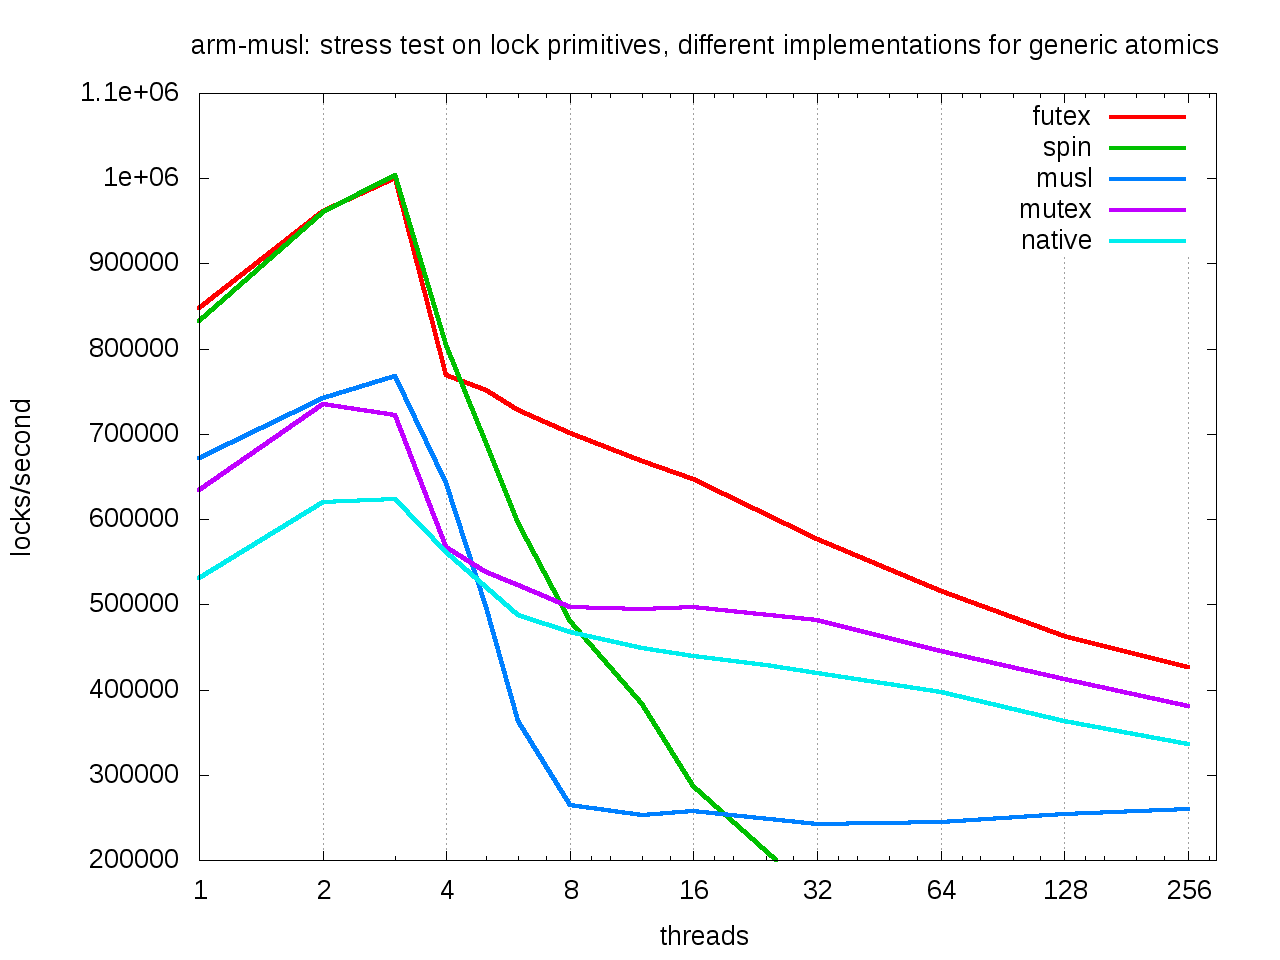
\includegraphics[width=0.48\textwidth]{benchs/arm/test-arm-u64.png}
  }%
  \subfigure[relative performance compared to mutex\label{fig:arm-rel}]{
    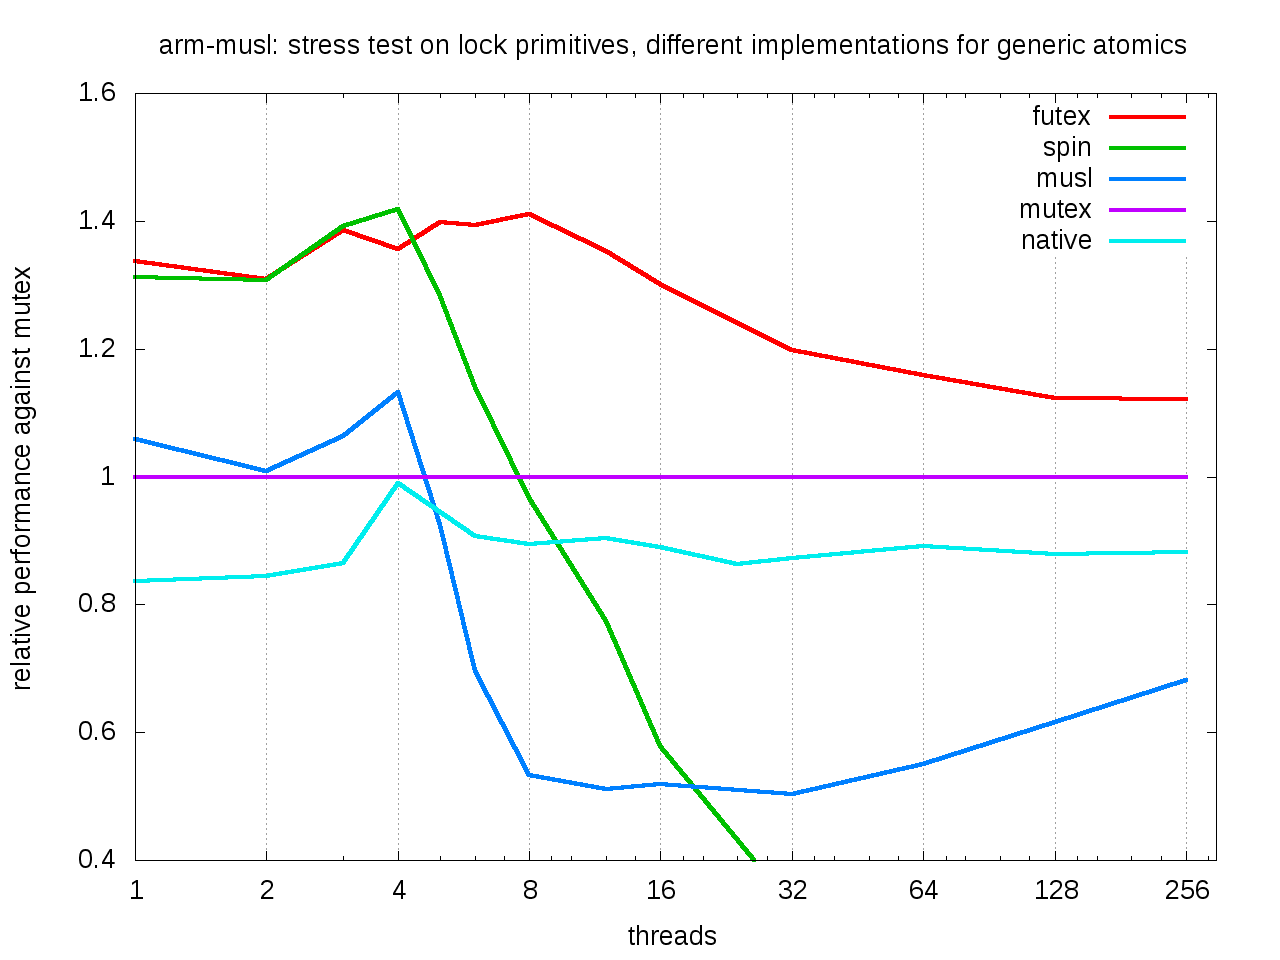
\includegraphics[width=0.48\textwidth]{benchs/arm/test-arm-u64-relative.png}
  }
  \caption{benchmarks on \texttt{arm}}
  \label{fig:arm}
\end{figure*}

\subsubsection{An \texttt{arm7} machine with 4 cores}
\label{sec-4-3-1}

This machine has 4 symmetric \texttt{arm7} cores at a \texttt{1.3 GHz} with \texttt{2
    GiB} of RAM. This system is equipped with Alpine Linux, so it has
\texttt{musl} as a native C library. The processor has atomic
instructions for word sizes up to 64 bit. The compiler is \texttt{gcc}
version \texttt{4.9}.

\subsubsection{A \texttt{x86\_64} machine with 2x2 hyperthreaded cores}
\label{sec-4-3-2}

This is a i7-4600U CPU at \texttt{2.10GHz} and with \texttt{8 GiB} of RAM. The
OS is Debian Linux, with \texttt{glibc} as native library.  The processor
has atomic instructions for word sizes up to 128 bit. The compiler
is \texttt{gcc} version \texttt{5.2}.

\subsection{Performance comparison}
\label{sec-4-4}

The Fig.~\ref{fig:arm} shows the results on the \texttt{arm}
platform.
%
We see that all lock implementations allow for an acceleration of
the application when a small number of threads is used. But what is
also clear that the "native" lock performs worst for the case that
is the most interesting: the range where each thread has
its own CPU core at its disposal. Even the "mutex" lock performs better.

We also see that musl's internal lock structure shows a drastic
performance loss when it comes to congestion. This is due to a
switch of the spinning strategy: as soon as congestion is detected,
spinning is abandoned and threads directly attempt
\code{futex_wait}. This is meant to ensure fairness of lock acquisition,
but as we can see for our use case it has a dramatic impact on the
application throughput.

Here is the relative performance of the same experiments, where the
"mutex" implementation is taken as a base:

We see that our new implementation is about 60\% better than
the "native" version, or 40\% than a direct implementation with
mutex. It combines the good performance of a spinlock for the less
congested range with a good policy for strong congestion.

To finish let us consider the \texttt{x86\_64} platform. Although it
is much more powerful than the other, the atomics of the hardware
are much less performing. This is due to the fact that here an
atomic instruction almost always enforces a complete
synchronization. So any atomic operation incurs a strong latency
penalty. Thereby, our application is not even able to accelerate for
2, 3 or 4 threads as it was the case on arm. In the contrary it
even decelerates.
Nevertheless the relative performance difference between the
different lock implementations look very similar.%
\iflong
\begin{figure*}[t]
  \subfigure[lock throughput\label{fig:x86_64-abs}
  ]{
    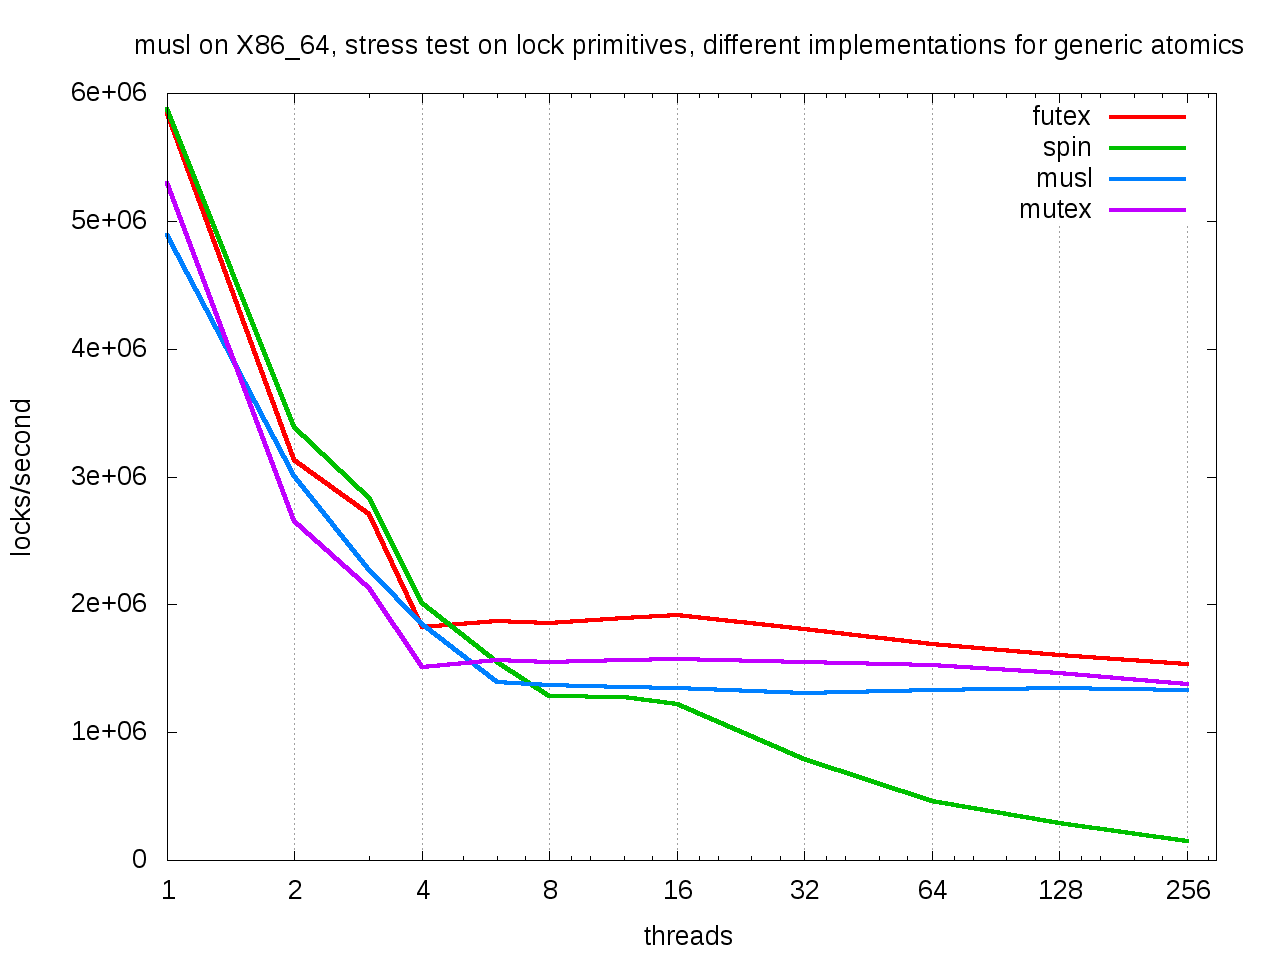
\includegraphics[width=0.48\textwidth]{benchs/x86_64/test-x86_64-musl.png}
  }%
  \subfigure[relative performance compared to mutex\label{fig:x86_64-rel}]{
    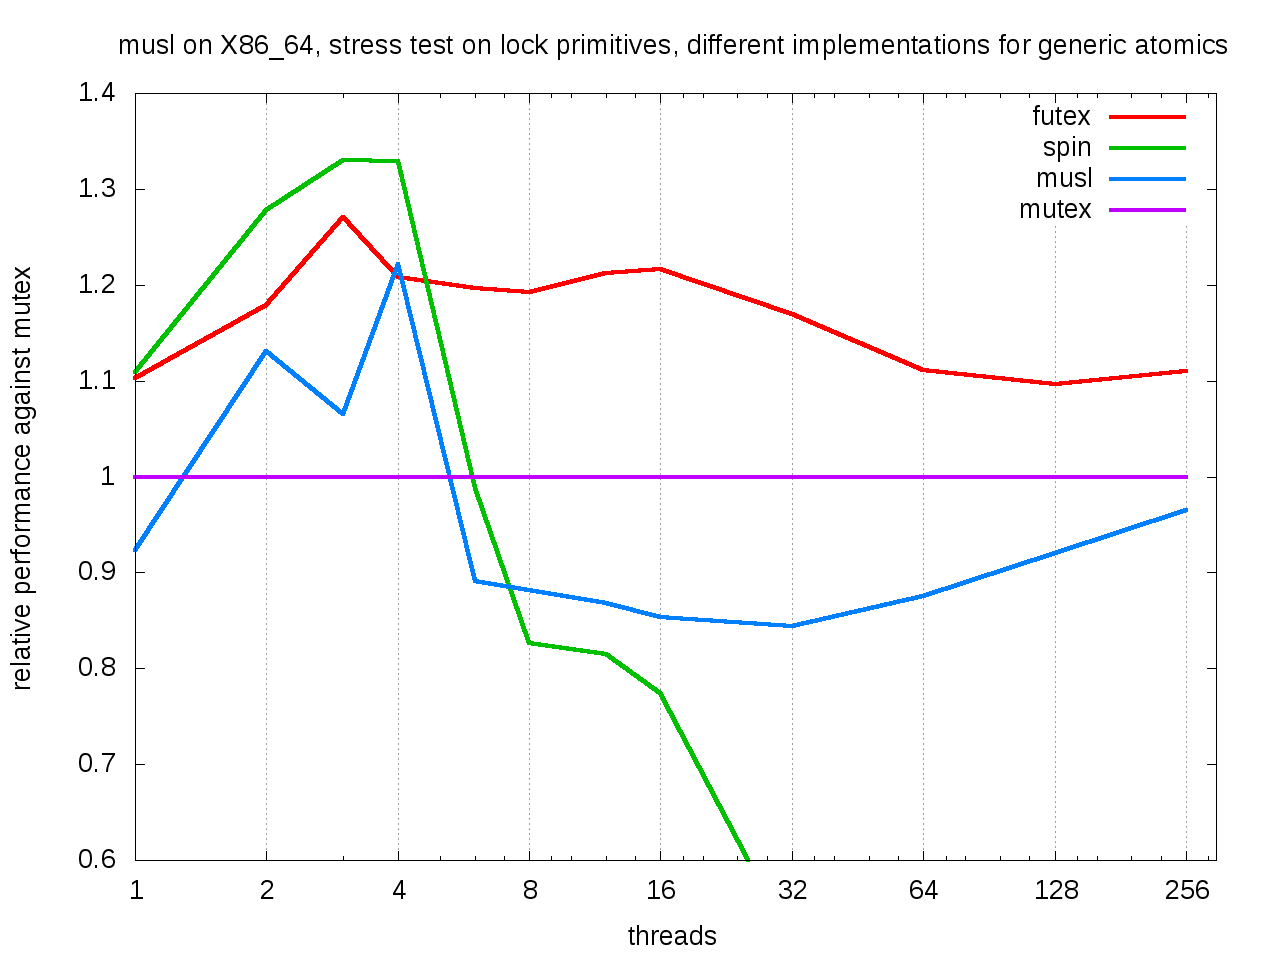
\includegraphics[width=0.48\textwidth]{benchs/x86_64/test-x86_64-musl-relative.png}
  }
  \caption{benchmarks on \texttt{x86\_64}}
  \label{fig:x86_64}
\end{figure*}
\else
\footnote{Figures not shown, due to space limitations.}
\fi

\section{Conclusion}
\label{sec-5}

We have presented a new locking algorithm that combines consequent use
of C11 atomics with Linux' futex system calls. We have proven that it
is deadlock free.

When compared to other lock implementations it shows better
performance. This is not surprising, an implementation that is tuned
for the purpose (very short CS) and that may avoid stacked calls into
the C library should always perform better than a generic one.
Surprising to us was the wide performance gap between the
implementations.

By pursuing this research we also learned to mistrust some of the
urban legends that turn around atomics, futexes and lock structures in
general. At least when we stick to the basics (\code{futex_wait} and
\code{futex_wake}) and if we have a decent interface for atomics,
programming them is not as difficult as the legends suggest. Also
using a system call is not so much worse that spinning around an
atomic access. The performance factor between the two is only about
10, and so spinlocks in the order of 10 should be sufficient in many
cases.

In the future we plan to make this whole support library available as
open source project. We hope to integrat it into the C library that we
used for most of our experiments, \texttt{musl}.


%%% Local Variables:
%%% mode: latex
%%% mode: reftex
%%% fill-column: 75
%%% ispell-dictionary: "american"
%%% x-symbol-8bits: nil
%%% End:



%    Bibliography styles amsplain or harvard are also acceptable.
%\nocite{*}
%\bibliographystyle{ACM-Reference-Format-Journals}
%\bibliography{modernC}

%%% -*-BibTeX-*-
%%% Do NOT edit. File created by BibTeX with style
%%% ACM-Reference-Format-Journals [18-Jan-2012].

\begin{thebibliography}{00}

%%% ====================================================================
%%% NOTE TO THE USER: you can override these defaults by providing
%%% customized versions of any of these macros before the \bibliography
%%% command.  Each of them MUST provide its own final punctuation,
%%% except for \shownote{}, \showDOI{}, and \showURL{}.  The latter two
%%% do not use final punctuation, in order to avoid confusing it with
%%% the Web address.
%%%
%%% To suppress output of a particular field, define its macro to expand
%%% to an empty string, or better, \unskip, like this:
%%%
%%% \newcommand{\showDOI}[1]{\unskip}   % LaTeX syntax
%%%
%%% \def \showDOI #1{\unskip}           % plain TeX syntax
%%%
%%% ====================================================================

\ifx \showCODEN    \undefined \def \showCODEN     #1{\unskip}     \fi
\ifx \showDOI      \undefined \def \showDOI       #1{{\tt DOI:}\penalty0{#1}\ }
  \fi
\ifx \showISBNx    \undefined \def \showISBNx     #1{\unskip}     \fi
\ifx \showISBNxiii \undefined \def \showISBNxiii  #1{\unskip}     \fi
\ifx \showISSN     \undefined \def \showISSN      #1{\unskip}     \fi
\ifx \showLCCN     \undefined \def \showLCCN      #1{\unskip}     \fi
\ifx \shownote     \undefined \def \shownote      #1{#1}          \fi
\ifx \showarticletitle \undefined \def \showarticletitle #1{#1}   \fi
\ifx \showURL      \undefined \def \showURL       #1{#1}          \fi

\bibitem[\protect\citeauthoryear{Alpine}{Alpine}{}]%
        {alpine}
{Alpine}.
\newblock
\showURL{%
\url{http://alpinelinux.org/}}


\bibitem[\protect\citeauthoryear{Clang}{Clang}{}]%
        {clang}
{Clang}.
\newblock
\showURL{%
\url{http://clang.llvm.org/}}


\bibitem[\protect\citeauthoryear{Drepper}{Drepper}{2011}]%
        {drepper11:futex}
{Ulrich Drepper}. 2011.
\newblock Futexes are tricky.
\newblock Red Hat Inc., rev. 1.6.   (2011).
\newblock
\showURL{%
\url{http://www.akkadia.org/drepper/futex.pdf}}


\bibitem[\protect\citeauthoryear{gcc}{gcc}{}]%
        {gcc}
{gcc}.
\newblock {G}{N}{U} Compiler Collection.
\newblock
\showURL{%
\url{https://gcc.gnu.org/}}


\bibitem[\protect\citeauthoryear{glibc}{glibc}{}]%
        {glibc}
{glibc}.
\newblock {G}{N}{U} {C} library.
\newblock
\showURL{%
\url{https://www.gnu.org/software/libc/}}


\bibitem[\protect\citeauthoryear{Gustedt}{Gustedt}{2016}]%
        {gustedt16:futex}
{Jens Gustedt}. 2016.
\newblock \showarticletitle{Futex based locks for C11's generic atomics,
  extended abstract}. In {\em Proceedings of the 31st Annual ACM Symposium on
  Applied Computing}. ACM.
\newblock
\newblock
\shownote{accepted for publication.}


\bibitem[\protect\citeauthoryear{Hart}{Hart}{2009}]%
        {hart09}
{Darren Hart}. 2009.
\newblock \showarticletitle{A futex overview and update}.
\newblock {\em LWN.net\/} (2009).
\newblock
\showURL{%
\url{https://lwn.net/Articles/360699/}}


\bibitem[\protect\citeauthoryear{Hutton, Donovan, Ross, Franke, Russell, and
  Kirkwood}{Hutton et~al\mbox{.}}{2002}]%
        {Hutton02fuss}
{Andrew~J. Hutton}, {Stephanie Donovan}, {C.~Craig Ross}, {Hubertus Franke},
  {Rusty Russell}, {and} {Matthew Kirkwood}. 2002.
\newblock \showarticletitle{Fuss, Futexes and Furwocks: Fast Userlevel Locking
  in Linux}. In {\em Proceedings of the Ottawa Linux Symposium}. 479--495.
\newblock
\showURL{%
\url{https://www.kernel.org/doc/ols/2002/ols2002-pages-479-495.pdf}}


\bibitem[\protect\citeauthoryear{IBM}{IBM}{1983}]%
        {IBM370}
IBM 1983.
\newblock {\em IBM System/370 Extended Architecture, Principles of Operation}.
\newblock IBM.
\newblock
\newblock
\shownote{SA22-7085.}


\bibitem[\protect\citeauthoryear{JTC1/SC22/WG14}{JTC1/SC22/WG14}{2011}]%
        {C11}
{JTC1/SC22/WG14} (Ed.). 2011.
\newblock {\em Programming languages - {C}\/} (cor. 1:2012 ed.).
\newblock Number ISO/IEC 9899. ISO.
\newblock
\showURL{%
\url{http://www.open-std.org/jtc1/sc22/wg14/www/docs/n1570.pdf}}


\bibitem[\protect\citeauthoryear{Michael}{Michael}{2004}]%
        {michael04:aba}
{Maged~M. Michael}. 2004.
\newblock {\em {A}{B}{A} Prevention Using Single-Word Instructions}.
\newblock {T}echnical {R}eport RC23089. IBM Research.
\newblock


\bibitem[\protect\citeauthoryear{musl}{musl}{}]%
        {musl}
{musl}
\newblock libc.
\newblock
\showURL{%
\url{http://musl-libc.org}}


\bibitem[\protect\citeauthoryear{Netzer and Miller}{Netzer and Miller}{1992}]%
        {Netzer1992}
{Robert H.~B. Netzer} {and} {Barton~P. Miller}. 1992.
\newblock \showarticletitle{What Are Race Conditions? Some Issues and
  Formalizations}.
\newblock {\em ACM Lett. Program. Lang. Syst.\/} {1}, 1 (March 1992), 74--88.
\newblock
\showISSN{1057-4514}
\showDOI{%
\url{http://dx.doi.org/10.1145/130616.130623}}


\bibitem[\protect\citeauthoryear{POSIX}{POSIX}{2009}]%
        {POSIX2009}
{POSIX}. 2009.
\newblock {\em ISO/IEC/IEEE Information technology -- Portable Operating
  Systems Interface (POSIX®) Base Specifications}. Vol. 9945:2009.
\newblock ISO, Geneva, Switzerland.
\newblock
\newblock
\shownote{Issue 7.}


\end{thebibliography}


\end{document}

%%% Local Variables:
%%% mode: latex
%%% mode: reftex
%%% fill-column: 75
%%% ispell-dictionary: "american"
%%% x-symbol-8bits: nil
%%% End:
